%LAB4
\chapter{Punkt 5}

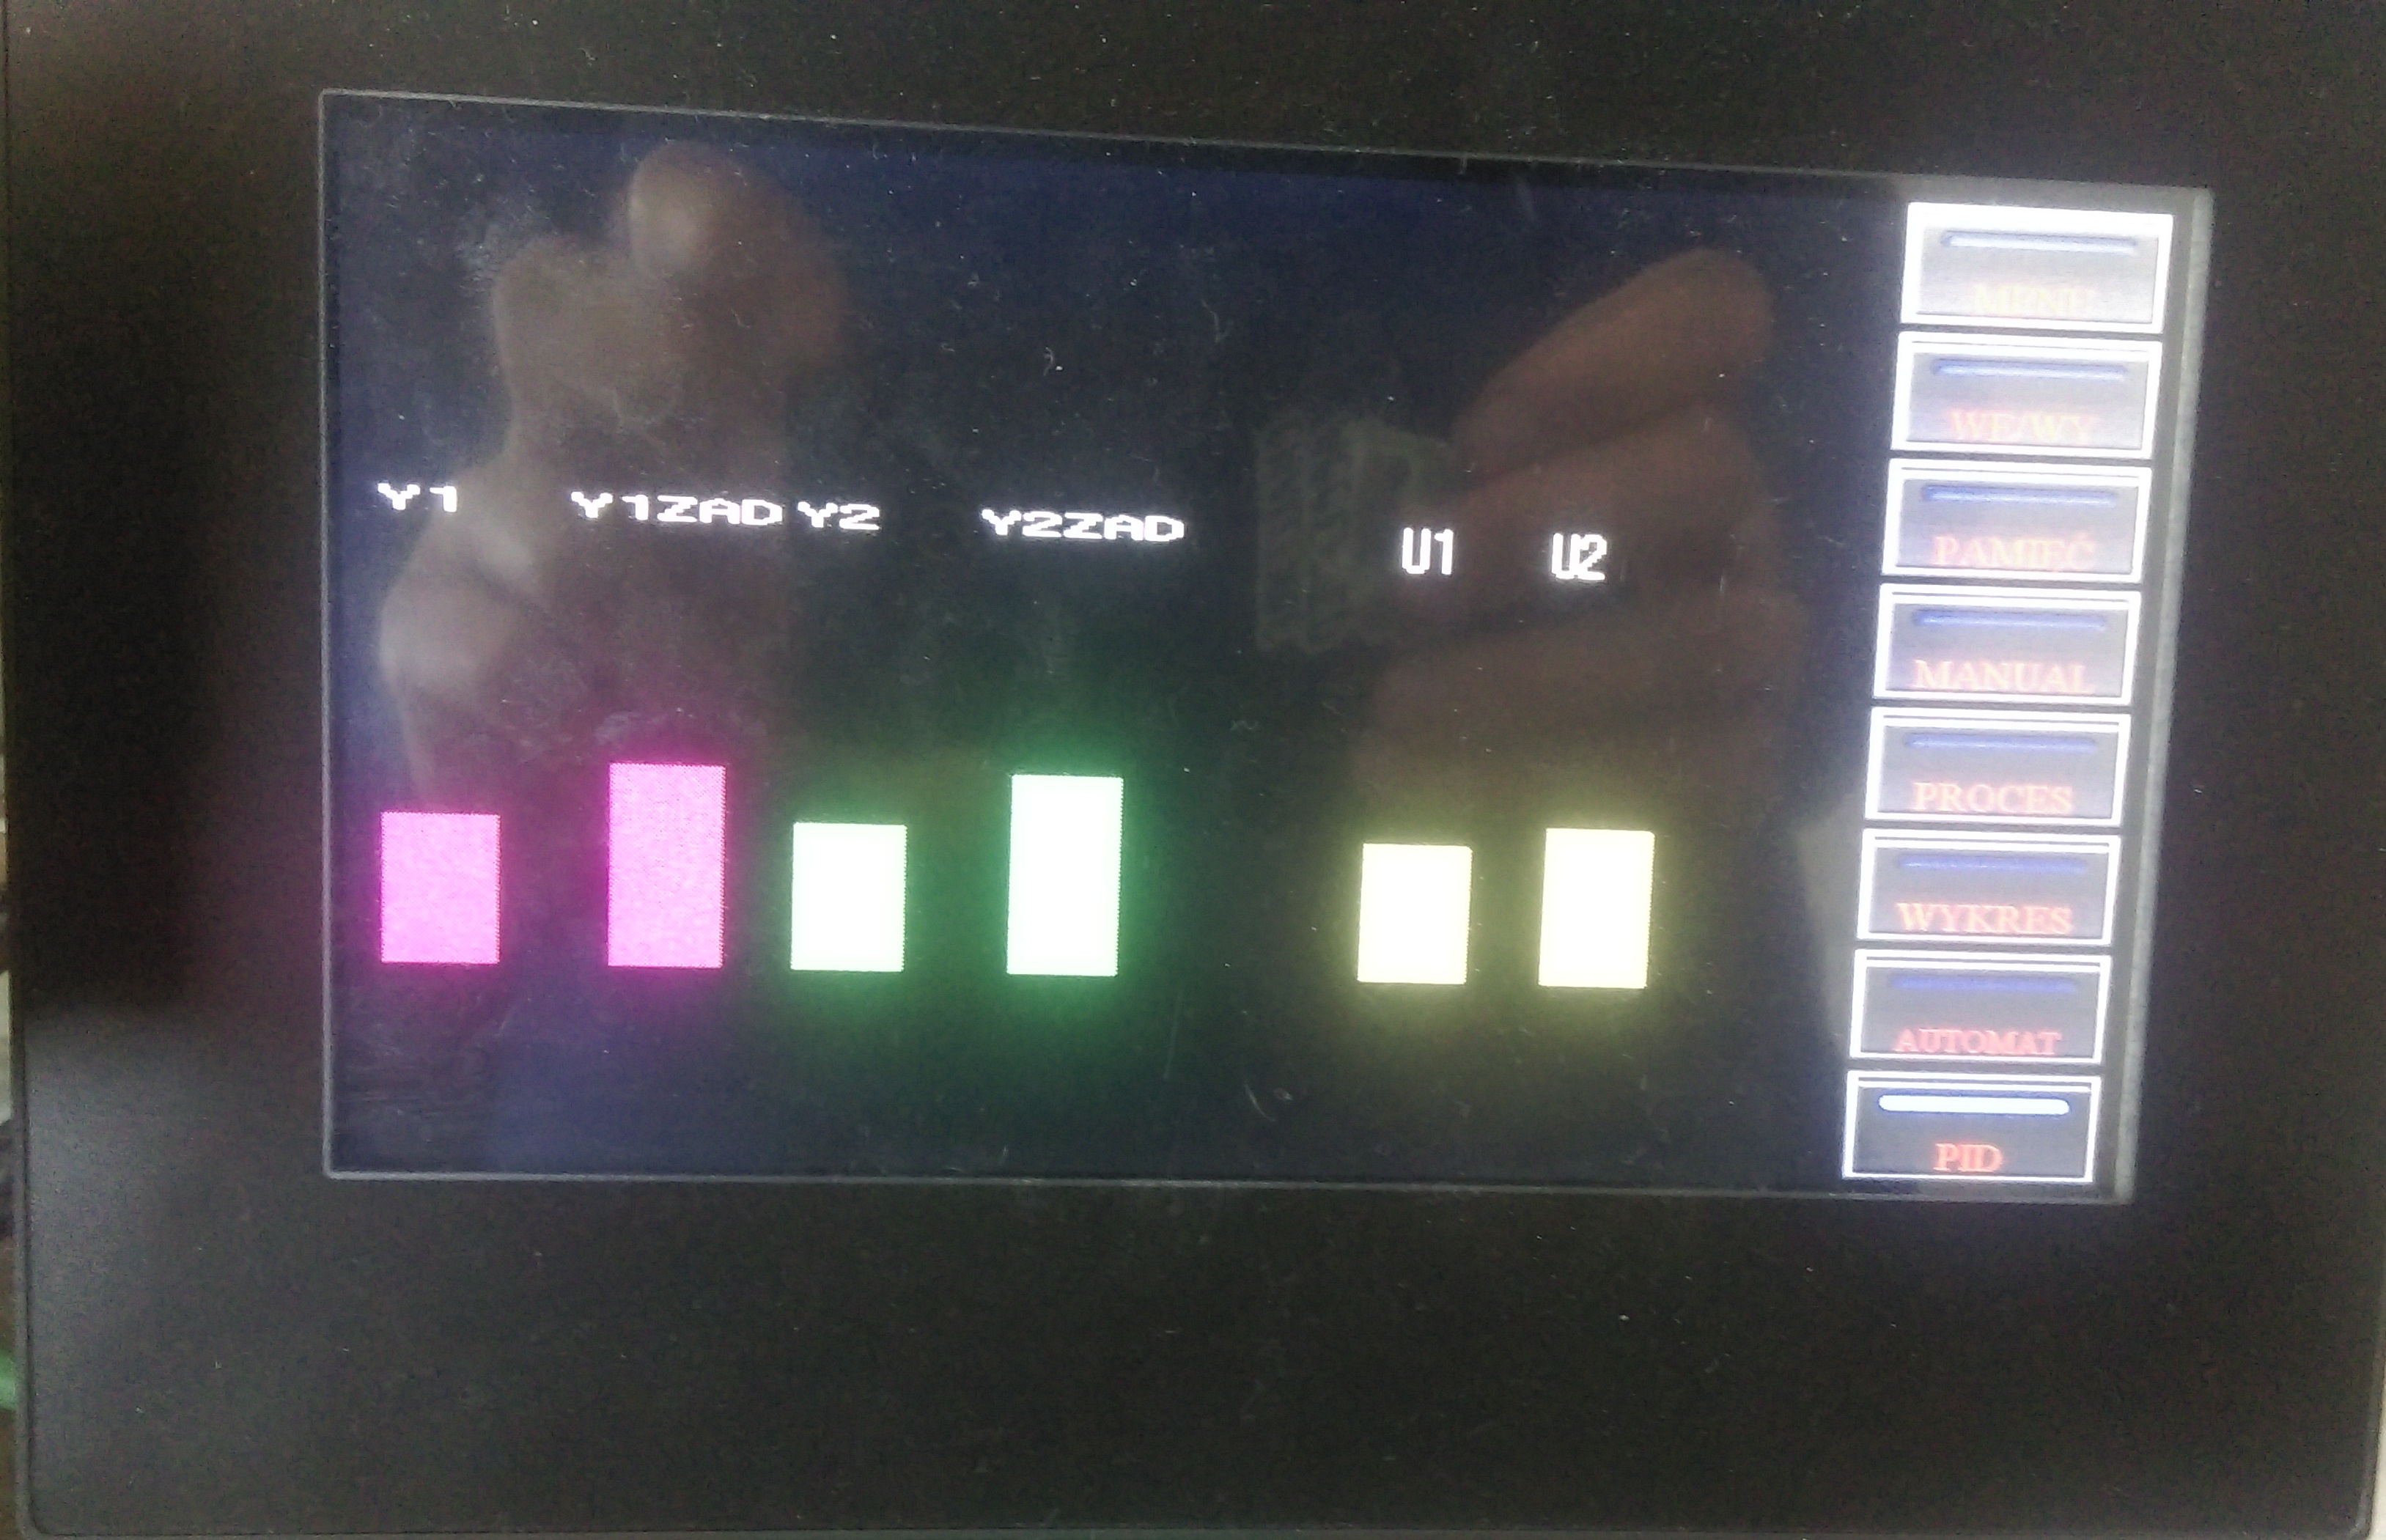
\includegraphics[width=6.1in]{Zadanie5}


Zaprojektowali�my prosty interfejs u�ytkownika do monitorowania stanowiska grzej�co ch�odz�cego.\\\\

Od lewej: \\\\
Kolor r�owy Y1 - pomiar temperatury T1, zakres: ($\num{0}\degree$C - pusty s�upek, $\num{100}\degree$C - pe�ny s�upek) \\
Kolor r�owy Y1ZAD - warto�� zadana temperatury T1, zakres j.w.\\
Kolor zielony Y2 - pomiar temperatury T3, zakres: ($\num{0}\degree$C - pusty s�upek, $\num{100}\degree$C - pe�ny s�upek) \\
Kolor zileony Y2ZAD - warto�� zadana temperatury T2, zakres j.w.\\
Kolor ��ty U1 - warto�c sterowania podana na grza�k� G1, zakres (0 \% - pusty s�upek, 100 \% - pe�ny s�upek)\\
Kolor ��ty U2 - warto�c sterowania podana na grza�k� G2, zakres (0 \% - pusty s�upek, 100 \% - pe�ny s�upek)\\\\

Panel jest dost�pny po wci�ni�cu po prawej stronie przycisku MENU, a nast�pnie przycisku PID.\\